\documentclass[12pt,a4paper,oneside]{ctexart}
\usepackage{amsmath,amsthm,amssymb,CJK,wrapfig,graphicx,float,tabularx}
\title{液体表面张力实验报告}
\author{张博厚 PB22071354}
\date{2023.6.12}
\begin{document}
\maketitle
\tableofcontents
\newpage
\section{实验背景}
表面张力,是指液体表面层由于分子引力不均衡而产生的沿表面作用于任一界线上的张力.
这种力在宏观上使得液体尽量收缩其表面,如同一张绷紧的弹性膜一样.
\par 实验表明,在液体表面上取一条虚拟的线段,
该线段两边液面间的表面张力$f$与线段长度$l$成正比,即
\begin{equation}
    f=\sigma l
\end{equation}
其中$\sigma$称为表面张力系数,其大小与液体的成分,纯度,浓度,温度均有关.本实验采用
焦利氏秤法(拉脱法),用秤量仪器直接测量液体的表面张力,直接清楚.
\section{实验原理与方法}
\subsection{实验原理}
本实验所采用的的主要仪器为焦利氏秤,它实际上是一种用来测微小力的精细弹簧秤,通过
保持弹簧下端位置固定,向上拉动弹簧确定伸长值,进而计算拉力.
原理图如下:
\begin{figure}[H]
    \centering
    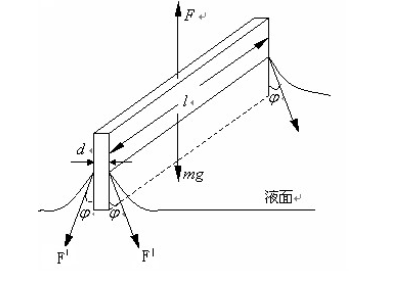
\includegraphics[scale=0.8]{原理图.png}
    \caption{实验原理}
\end{figure}
在金属丝框拉出水面的过程中,金属丝框在下面带起一水膜,当水膜恰好被拉断时,各力的平衡条件为:
\begin{equation}
    F=mg+2F'
\end{equation}
而\begin{equation}
    F'=\sigma l
\end{equation}
因此
\begin{equation}
    \sigma=\frac{F-mg}{2l}
\end{equation}
\subsection{实验装置}
焦利氏秤,砝码(0.5g-5g),钢板尺,烧杯,镊子,自来水与洗洁精,金属圈,金属丝
\subsection{实验内容/步骤}
\noindent
一.确定焦利氏秤上锥形弹簧的劲度系数
\begin{itemize}
    \item[] 
    (1) 组装焦利氏秤,依次安装弹簧,镜子,砝码盘.调节支架底座的螺丝使秤框竖直,
小镜子应正好位于玻璃管中间.\\
(2) 逐次在砝码盘内放入砝码,每次增量 0.5g 的砝码,从 0.5g~5g 范围内增加.每次操
作都要调节升降钮,做到三线合一,即玻璃圆筒上的刻线,小平面镜上的刻线,圆筒刻线在平面镜中的像对齐.
记录升降杆的位置读数,计算出弹簧的劲度系数.
\end{itemize}
二.用金属圈测量自来水的表面张力系数:
\begin{itemize}
    \item[] 
    (1) 测量金属圈的直径 d;\\
(2) 取下砝码,在砝码盘下挂上金属圈,保持三线合一,记下此时升降杆读数;\\
(3) 将盛有自来水的烧杯放在焦利氏秤台上,调节平台的微调螺丝和升降钮,使金属圈浸入水面以下;\\
(4) 缓慢地旋转平台微调螺丝和升降钮,注意烧杯下降和金属杆上升时,始终保持三线合一,
当液膜刚要破裂时,记下金属杆的读数.测量 5 次,取平均,计算自来水的表面张力系数,并计算不确定度.
\end{itemize}
三.用金属丝测量肥皂水的表面张力系数:
\begin{itemize}
    \item[] 
    (1) 测量金属丝两脚之间的距离 s;\\
    (2) 重复上述二中的步骤(2)-(4),计算肥皂水的表面张力系数.
\end{itemize}
四.用二中的方法,测量并计算自配洗洁精溶液的表面张力系数,并得出关系曲线.
\section{数据记录与处理}
\subsection{确定弹簧劲度系数}
砝码质量与弹簧长度的关系如下
\begin{center}
    \begin{tabular}{|c|c|c|c|c|c|c|c|c|c|c|c|}
    \hline
    质量m/g&0&0.5&1&1.5&2&2.5&3&3.5&4&4.5&5\\
    \hline
    距离x/cm&1.53&1.96&2.36&2.79&3.25&3.70&4.11&4.56&5.00&5.45&5.87\\
    \hline
    \end{tabular}
\end{center}
利用合肥本地重力加速度值$g=9.79$,计算G并作线性拟合图如下:
\begin{figure}[H]
    \centering
    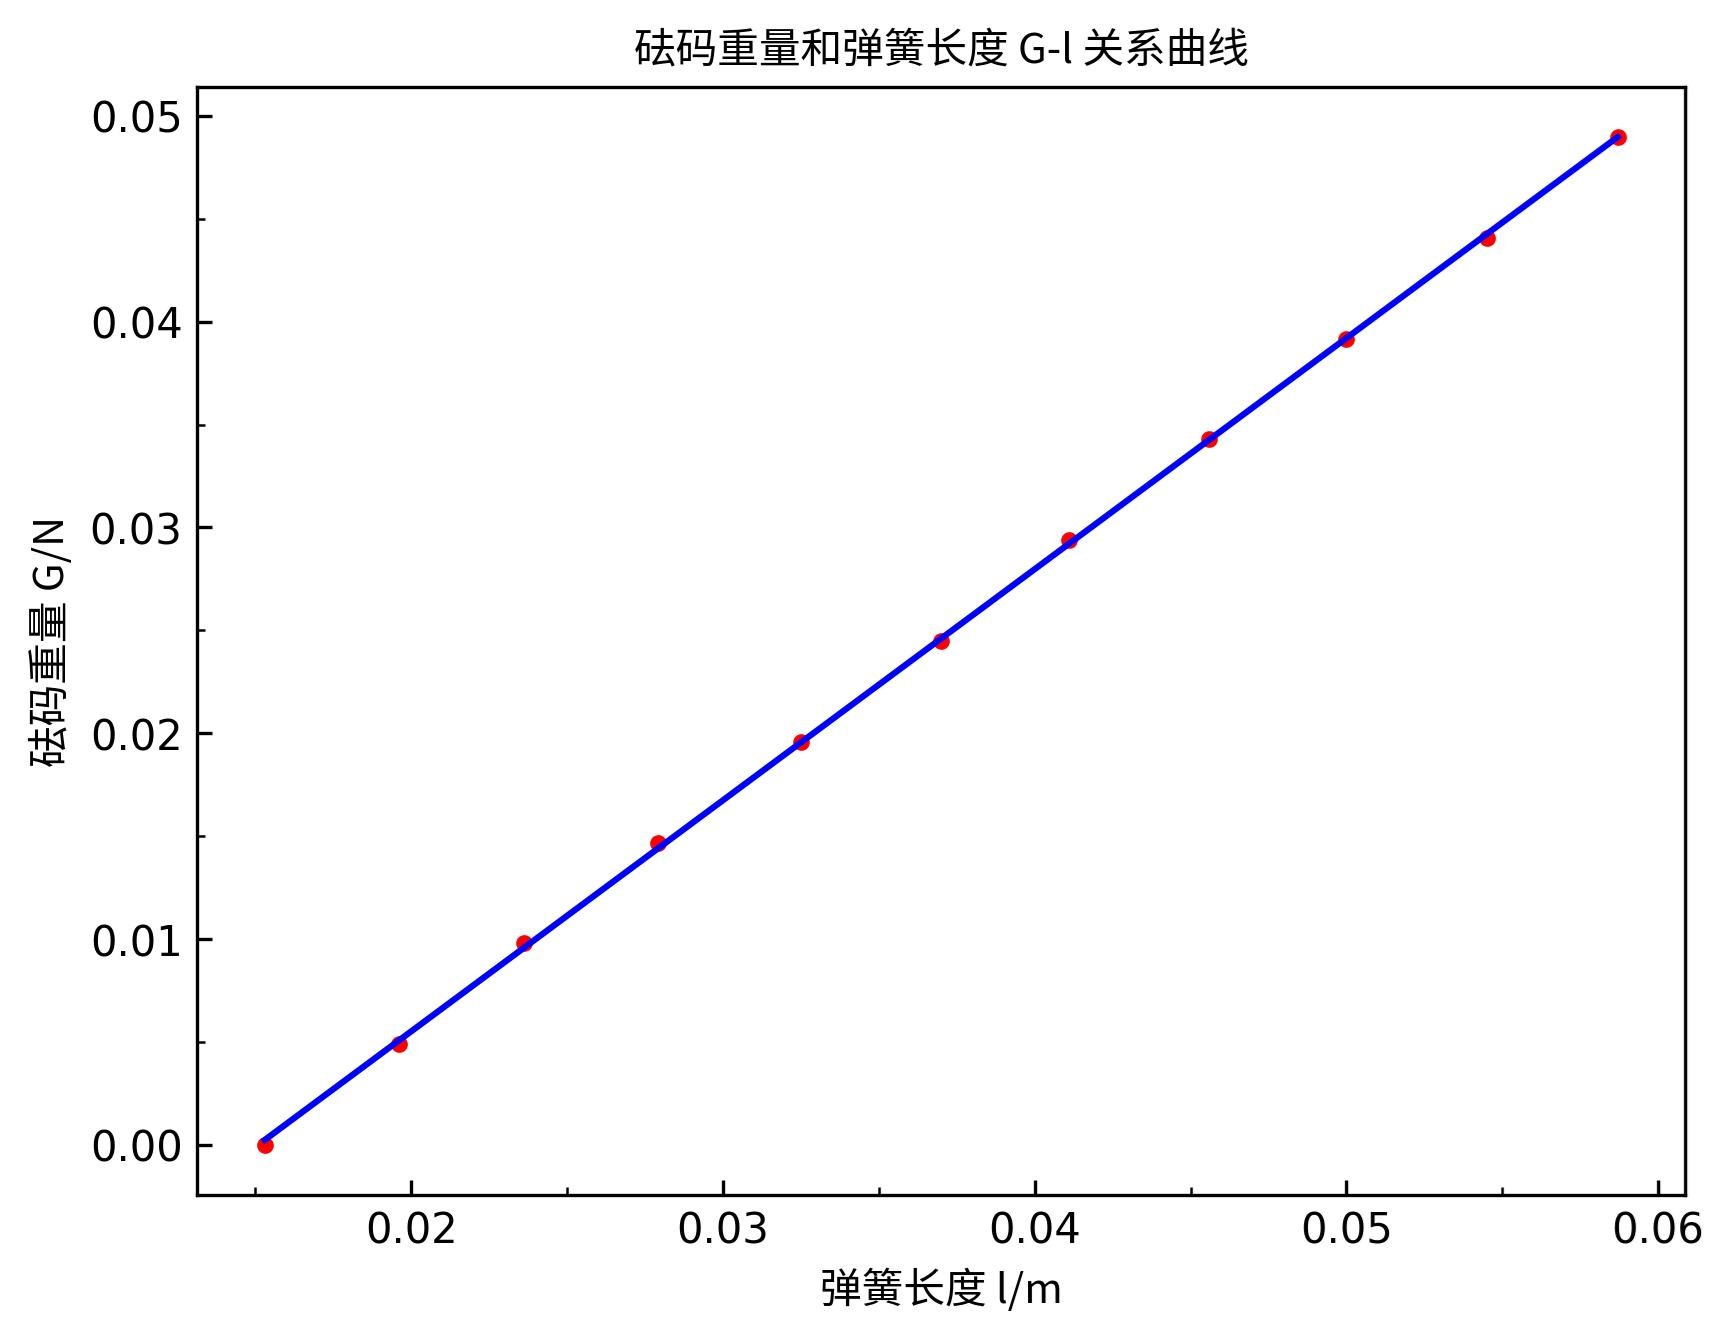
\includegraphics[scale=0.8]{最小二乘法拟合.jpg}
    \caption{最小二乘法拟合}
\end{figure}
\noindent
斜率
$$
m=1.1226\,\mathrm{N/m}
$$
截距
$$
b=-0.016929\,\mathrm{N}
$$
线性拟合的相关系数
$$
r=\frac{\overline{Fl}-\overline{F}\cdot\overline{l}}{\sqrt{\left(\overline{F^2}-\overline{F}^2\right)\left(\overline{l^2}-\overline{l}^2\right)}}=0.99994058
$$
故弹簧劲度系数为$k=1.1226N/m$
\subsection{用金属圈测量自来水的表面张力系数}
\noindent
原始数据见附录1:实验操作数据\\
铁丝圈直径d的平均值为
$$
\overline{d}=\frac{1}{n}\sum_{i=1}^{n}d_i=\frac{3.21+3.1+3.13}{3}\,\mathrm{cm}=3.1467\,\mathrm{cm}
$$
铁丝圈直径d的标准差
$$
\begin{aligned}
\sigma_{d}&=\sqrt{\frac{1}{n-1}\sum_{i=1}^n\left(d_i-\overline{d}\right)^2}\\
&=\sqrt{\frac{(3.21-3.1467)^2+(3.1-3.1467)^2+(3.13-3.1467)^2}{3-1}}\,\mathrm{cm}\\
&=0.056862\,\mathrm{cm}
\end{aligned}
$$
则其A类不确定度为
$$\Delta_{A,d}=\dfrac{\sigma_{d}}{\sqrt{n}}=0.032829cm$$
B类不确定度为
$$
\Delta_{B,d}=\sqrt{\Delta_\text{仪}^2+\Delta_\text{估}^2}=\sqrt{0.01^2+0.005^2}\,\mathrm{cm}=0.01118\,\mathrm{cm}
$$
展伸不确定度为
$$
\begin{aligned}
U_d&=\sqrt{\left(t_P\Delta_{A,d}\right)^2+\left(k_P\frac{\Delta_{B,d}}{C}\right)^2}\\
&=\sqrt{\left(4.3\times0.32829\right)^2+\left(1.96\times\frac{0.01118}{3}\right)^2}\,\mathrm{cm}\\
&=0.14136\,\mathrm{cm} \qquad (P=0.95)
\end{aligned}
$$

\noindent
弹簧伸长量Δl的平均值
$$
\overline{\Delta l}=\frac{1}{n}\sum_{i=1}^{n}\Delta l_i=\frac{1.02+1.04+1.1+1.04+1.06}{5}\,\mathrm{cm}=1.052\,\mathrm{cm}
$$
其标准差为
\begin{small}
$$
\begin{aligned}
\sigma_{\Delta l}&=\sqrt{\frac{1}{n-1}\sum_{i=1}^n\left(\Delta l_i-\overline{\Delta l}\right)^2}\\
&=\sqrt{\frac{(1.02-1.052)^2+(1.04-1.052)^2+(1.1-1.052)^2+(1.04-1.052)^2+(1.06-1.052)^2}{5-1}}\\
&=0.030332\,\mathrm{cm}
\end{aligned}
$$
\end{small}
则其A类不确定度为
$$\Delta_{A,\Delta l}=\dfrac{\sigma_{\Delta l}}{\sqrt{n}}=0.01356cm$$
B类不确定度为
$$
\Delta_{B,\Delta l}=\sqrt{\Delta_\text{仪}^2+\Delta_\text{估}^2}=\sqrt{0.01^2+0.005^2}\,\mathrm{cm}=0.01118\,\mathrm{cm}
$$
展伸不确定度为
$$
\begin{aligned}
U_{\Delta l}&=\sqrt{\left(t_P\Delta_{A,\Delta l}\right)^2+\left(k_P\frac{\Delta_{B,\Delta l}}{C}\right)^2}\\
&=\sqrt{\left(2.78\times0.01356\right)^2+\left(1.96\times\frac{0.01118}{3}\right)^2}\,\mathrm{cm}\\
&=0.038411\,\mathrm{cm} \qquad(P=0.95)
\end{aligned}
$$
在拉起过程中,由式(4),并根据$F-mg=k\Delta l$,知
\begin{equation}
    \sigma = \dfrac{k\Delta l}{\pi d}
\end{equation}
代入数据得
$$
\sigma=\frac{k \overline{\Delta l}}{\pi \overline{d}}=0.11946\,\mathrm{N/m}
$$
其展伸不确定度为
$$
\dfrac{U_{\sigma}}{\sigma}=\sqrt{\left(\frac{U_d}{\overline{d}}\right)^2
+\left(\frac{U_{\Delta l}}{\overline{l}}\right)^2}=0.05789
$$
$$
U_{\sigma}=0.05789\times0.11946N/m=6.916\times10^{-3}N/m$$
故
$$
\sigma=\left(0.119 \pm 0.0069\right)\,\mathrm{N/m}
$$
\subsection{用金属丝测量肥皂水的表面张力系数} \noindent
原始数据见附录1,有
$$\overline{s}=\dfrac{4.50+4.49+4.47}{3}cm=4.487cm$$
$$\overline{\Delta l}=\dfrac{0.23+0.20+0.20+0.21+0.22}{5}cm= 0.212cm$$
故
$$\sigma=\dfrac{k\overline{\Delta l}}{2\overline{s}}=0.027N/m$$
\subsection{测量不同浓度溶液的表面张力系数}
\begin{center}
    \begin{tabular}{|c|c|c|c|}
        \hline
        n&1&2&3\\
        \hline
        浓度比&100:1&200:3&80:3\\
        \hline
        $\Delta l/cm$&0.21&0.35&0.36\\
        \hline
    \end{tabular}
\end{center}
则浓度比为$100:1$时
$$\sigma_1=\dfrac{k\overline{\Delta l}_1}{2\overline{s}}=0.026N/m$$
浓度比为$200:3$时
$$\sigma_2=\dfrac{k\overline{\Delta l}_2}{2\overline{s}}=0.044N/m$$
浓度比为$80:3$时
$$\sigma_3=\dfrac{k\overline{\Delta l}_3}{2\overline{s}}=0.045N/m$$
\section{思考与讨论}
\subsection{焦利氏秤法测定液体表面张力有什么优点?}
\noindent
1.测量液体表面张力时,需要在液膜即将破裂时读数,普通的弹簧难以做到,而焦利氏秤固定下端,
通过拉伸上端来进行读数,更有利于找到临界状态.\\
2.通过秤量仪器直接测量,不需要复杂的公式推导,更加直观方便.\\
3.焦利氏秤测量的量程与分度小,精度高.\\
4.使用锥形弹簧,可拉伸程度小,能测量微小力,同时其锥形外形能消除自重的影响.
\subsection{焦利氏秤的弹簧为什么做成锥形?}
\noindent
可以消除弹簧自重对弹簧伸长量和弹性系数的影响,保证弹簧各点的伸长量一致.
\subsection{应注意那些地方来减小误差?}
\noindent
1.实验前需调整好仪器,调节底脚螺丝使秤框竖直,注意实验过程中小镜子不能与玻璃管摩擦,
防止摩擦力影响表面张力的测量.\\
2.实验中始终注意保持三线对齐.\\
3.调节旋钮时动作应缓慢,防止拉脱临界点判断不准造成误差.\\
4.自配溶液进行实验时,应注意先把溶液搅拌均匀.
\newpage
\section{附录:实验原始数据}
\end{document}